\providecommand{\main}{../../../..}
\documentclass[\main/dresen_thesis.tex]{subfiles}

\begin{document}
  As the dispersion is composed of fast and slow evaporating components, the drop casting process subdivides into two parts.
  The first, where the primary fast evaporating phase of the dispersion evaporates and the second where the slowly evaporating phase is genlty reduced.

  \subsubsection{First Stage: Fast Evaporating Component}
    \begin{figure}[tb]
      \centering
      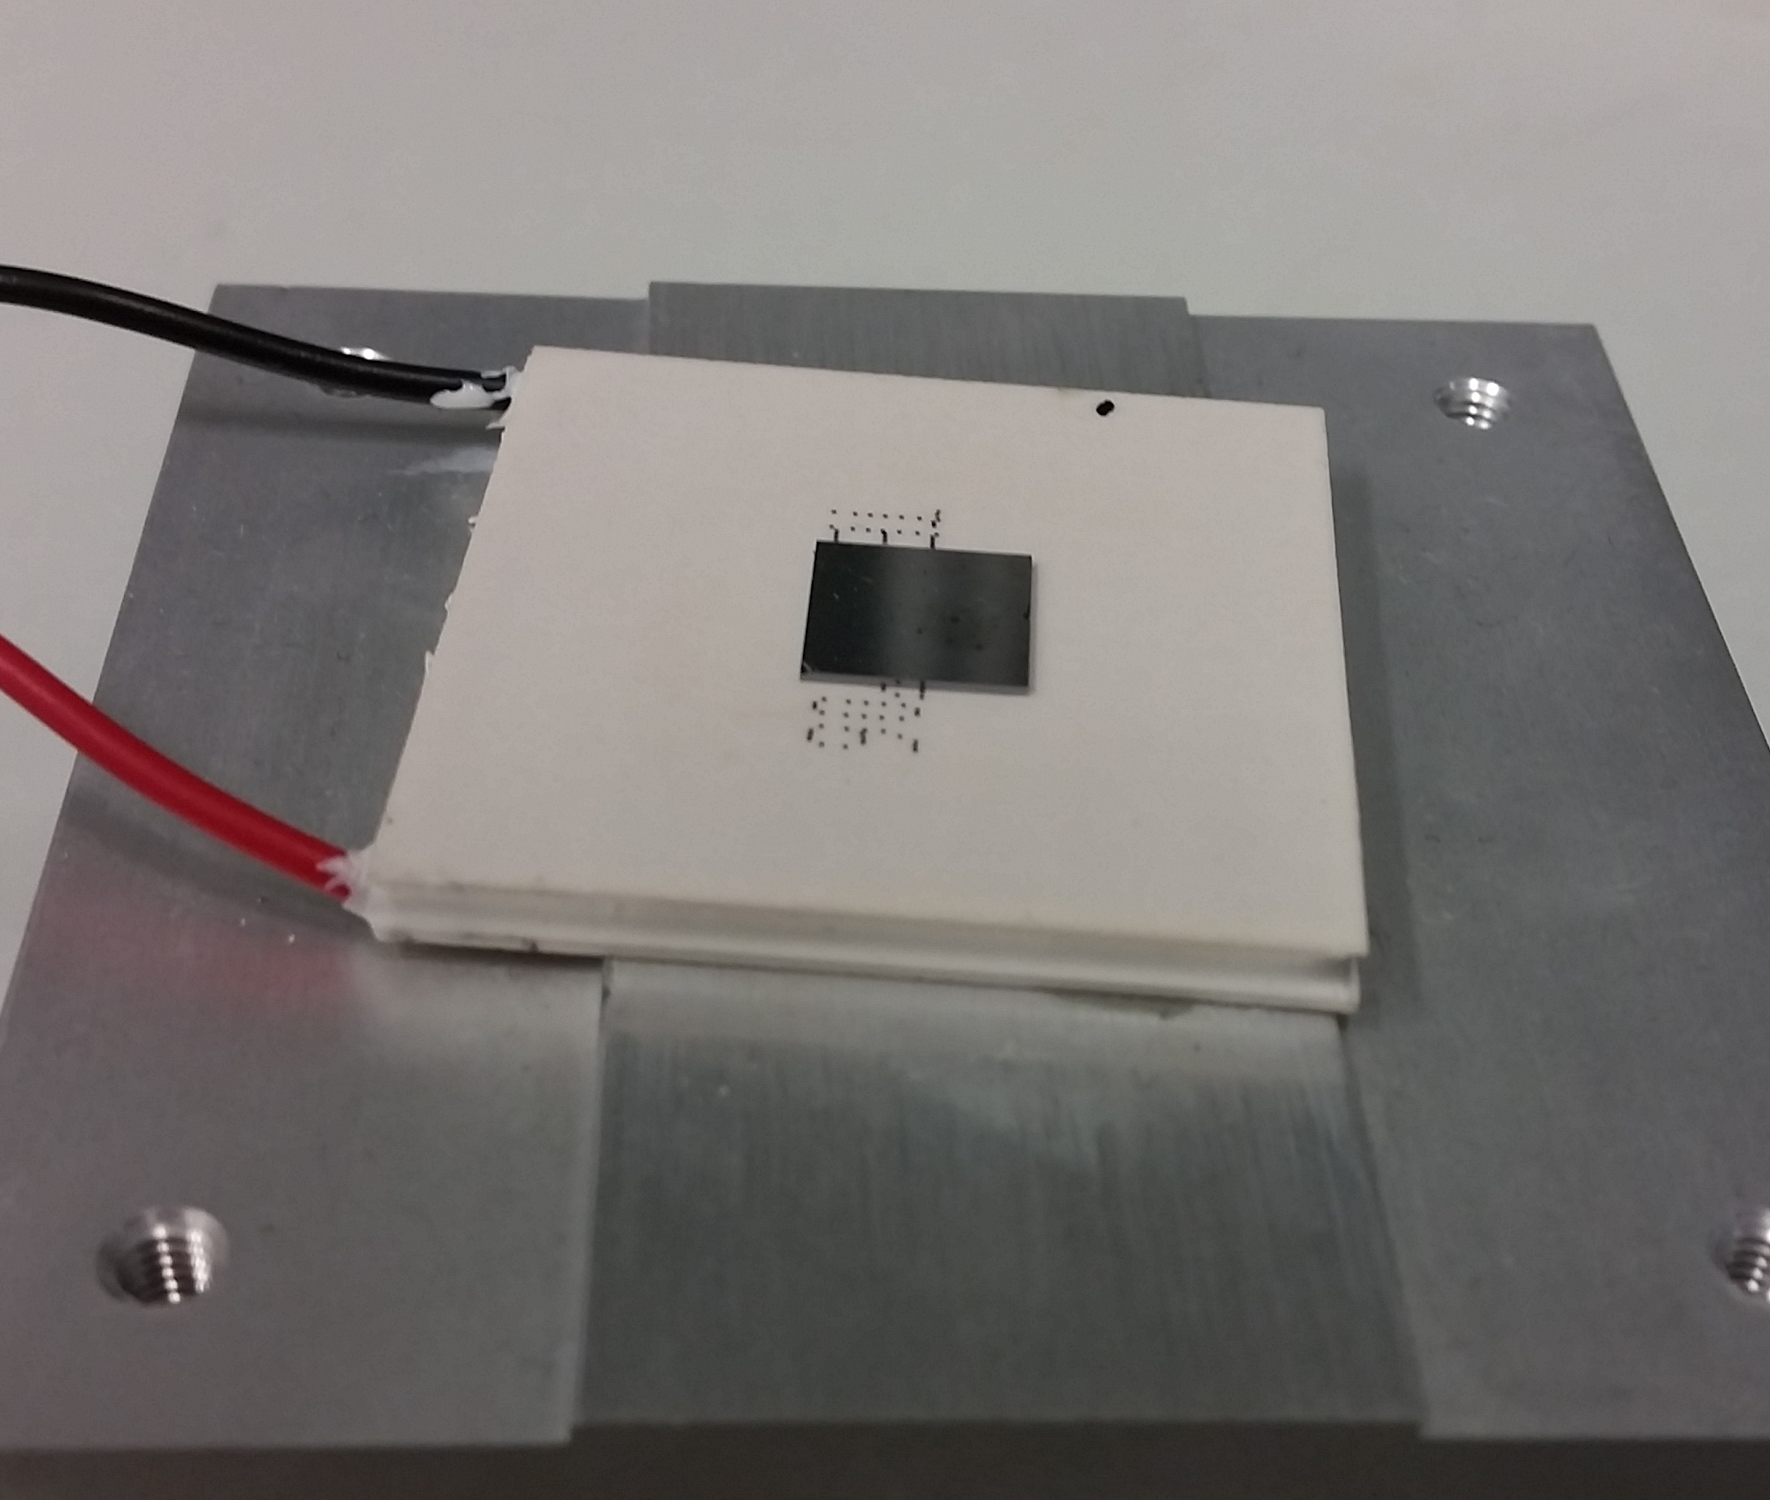
\includegraphics{monolayers_preparation_heating_stage}
      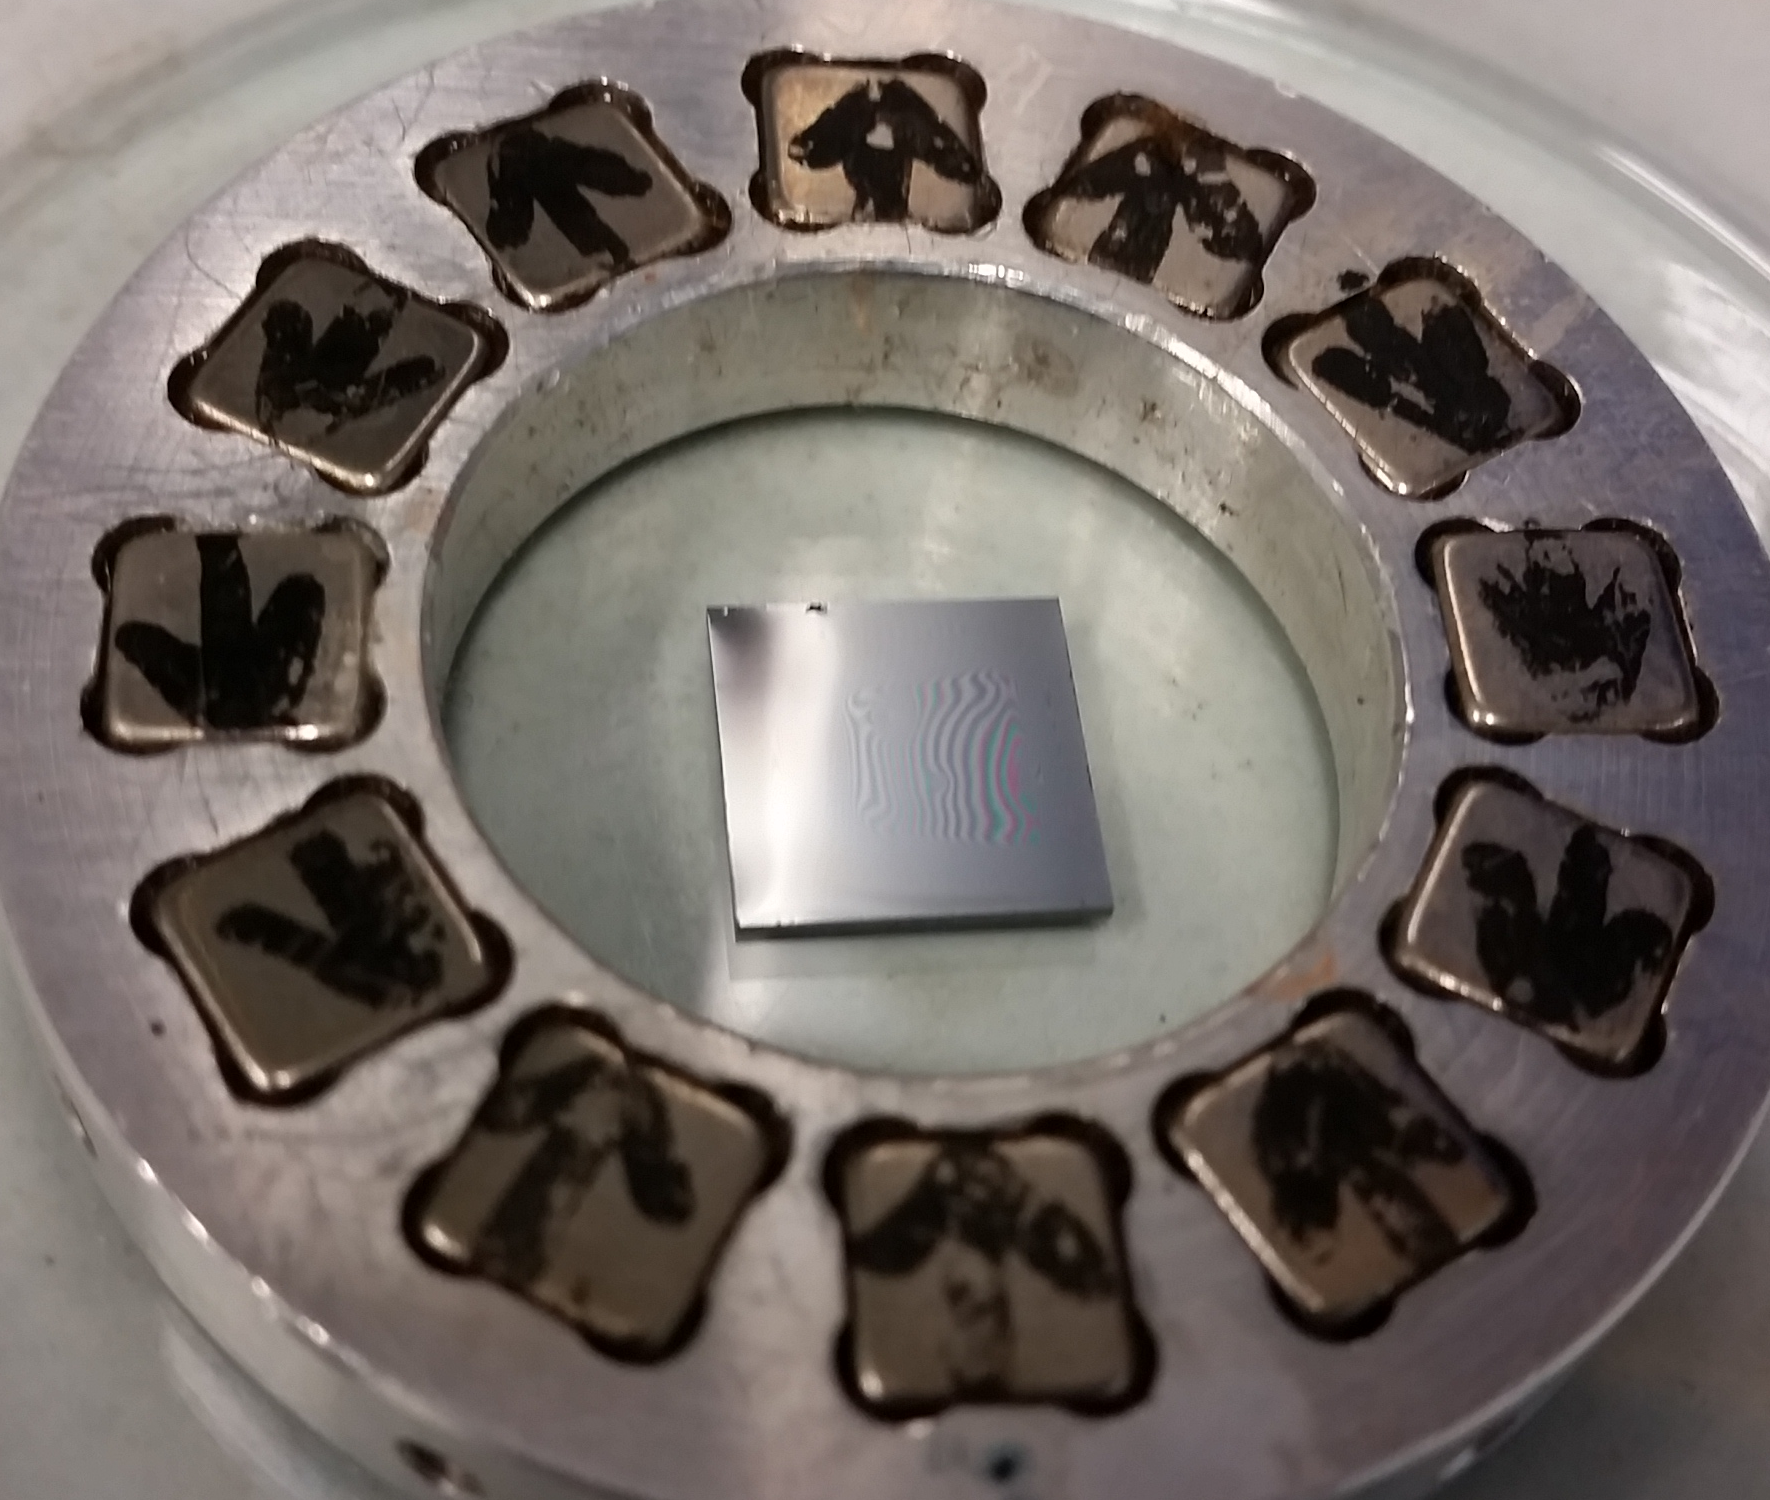
\includegraphics{monolayers_preparation_magnetic_field}
      \caption{\label{fig:monolayers:preparation:dryingConditions:varyConditions}The drying conditions for the droplet on the substrate can be varied continuously in temperature by means of a Peltier element (left) or an in-plane magnetic field can be added by using a Halbach cylinder (right).}
    \end{figure}  
    For the first part, different conditions were tested: the droplet was dried in an open container at ambient conditions ($T \eq 22 ^\circ C$), in a closed container with and without an additional solvent atmosphere, on a heating/cooling stage to change the surface temperature of the wafer (\reffig{fig:monolayers:preparation:dryingConditions:varyConditions}, left) or within an in-plane magnetic field (\reffig{fig:monolayers:preparation:dryingConditions:varyConditions}, right).
    Closing the container for the first evaporation step with and without solvent atmosphere, reduces the sample quality in the qualitative comparison of the SEM images to samples produced in open containers.
    As well as variation of the wafer temperature by the means of a Peltier element is not providing any improvement to the structure.
    When the wafer surface is cooled by applying a minimal voltage to the Peltier element, the 1-octadecene quickly freezes the complete dispersion at temperatures around $16 \unit{^\circ C}$ and no self-assembly process takes place.
    Increasing the temperature of the wafer on the other hand increases the inhomogeneity of the drying pattern.
    Both results obtained for the variation of the initial drying conditions support the kinetic theory of Bigioni \etal \cite{Bigioni_2006_Kinet} that the nanoparticles pin and self-assemble on the droplet surface as depicted in \reffig{fig:monolayers:preparation:dryingConditions:dryingStages}.
    For one, because the shrinking droplet height catches particles from the dispersion.
    And for the other, the nanoparticles stick there as the gentle cooling of the droplet surface through evaporative cooling increases the viscosity at the surface and handicaps the return of the particle from the surface to the bulk droplet.
    The attempted variations disturbed one or the other process and therefore reduced the achieved long range order quality of the obtained monolayers.
    \begin{figure}[tb]
      \centering
      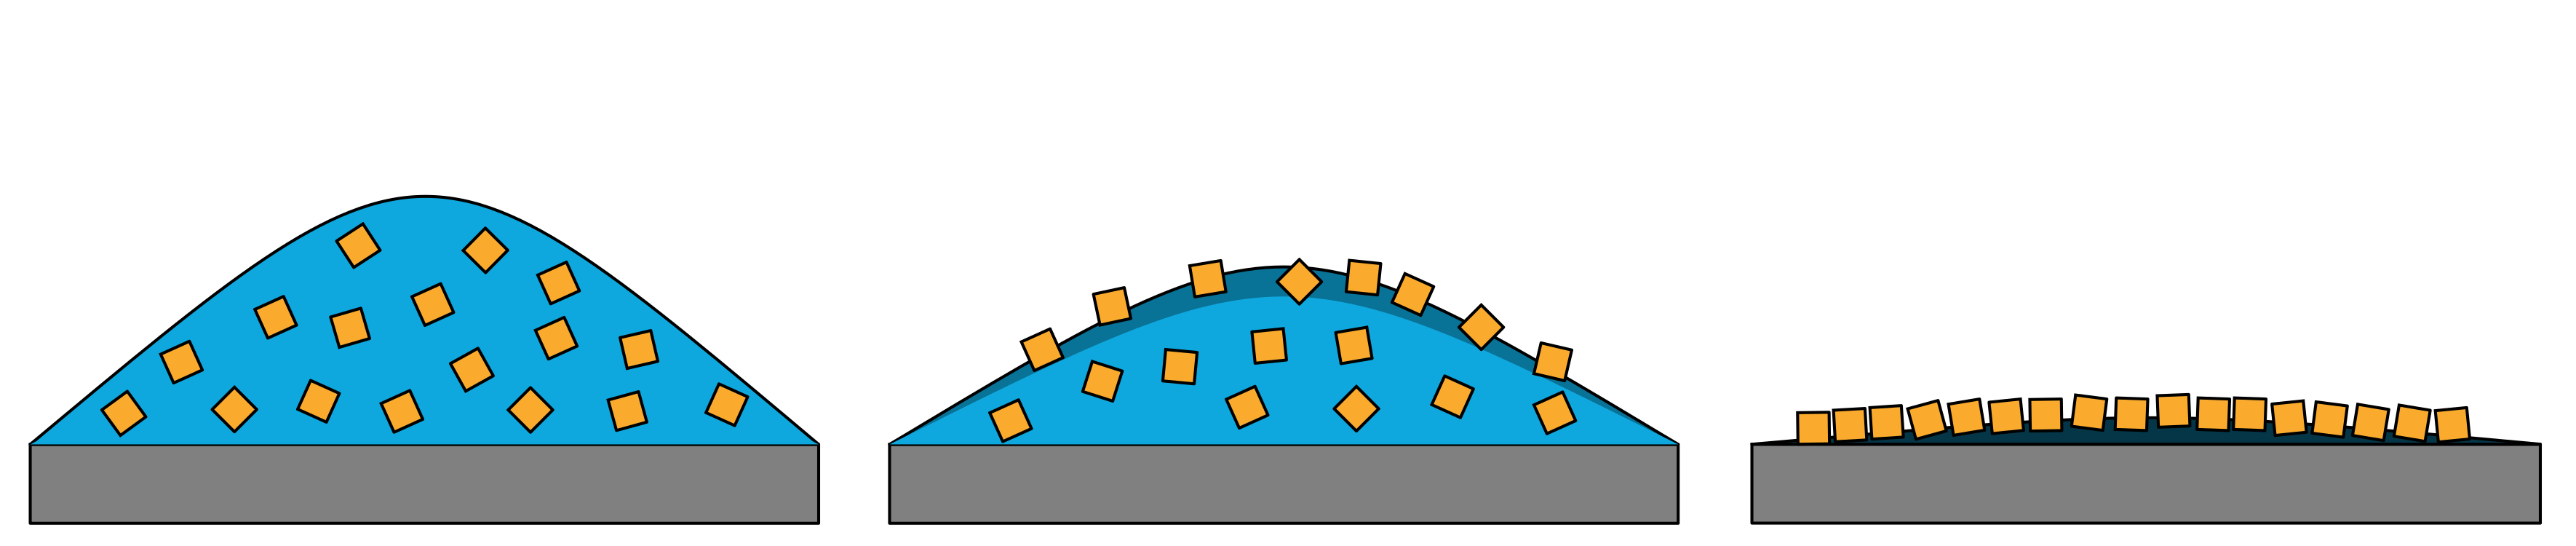
\includegraphics{monolayers_preparation_dryingStages}
      \caption{\label{fig:monolayers:preparation:dryingConditions:dryingStages} Depiction of the evolution during the first drying stage. As the droplet shrinks it fixes the nanoparticles on the droplet surface, where they can still move in two dimensions to form a long range ordered lattice. Finally the ordered structure remains with the remaining slow evaporating solvent.}
    \end{figure}

    Applying an in-plane magnetic field to strongly magnetic nanocubes during the first drying stages by the means of an Halbach cylinder, on the other hand, shows qualitatively a reduction of lattice defects and a tendency of aligning the cubes with the (100) faces along the magnetic field.
    This is visible by mere inspection from SEM shown in \reffig{fig:monolayers:preparation:dryingConditions:magneticField}.
    \begin{figure}[tb]
      \centering
      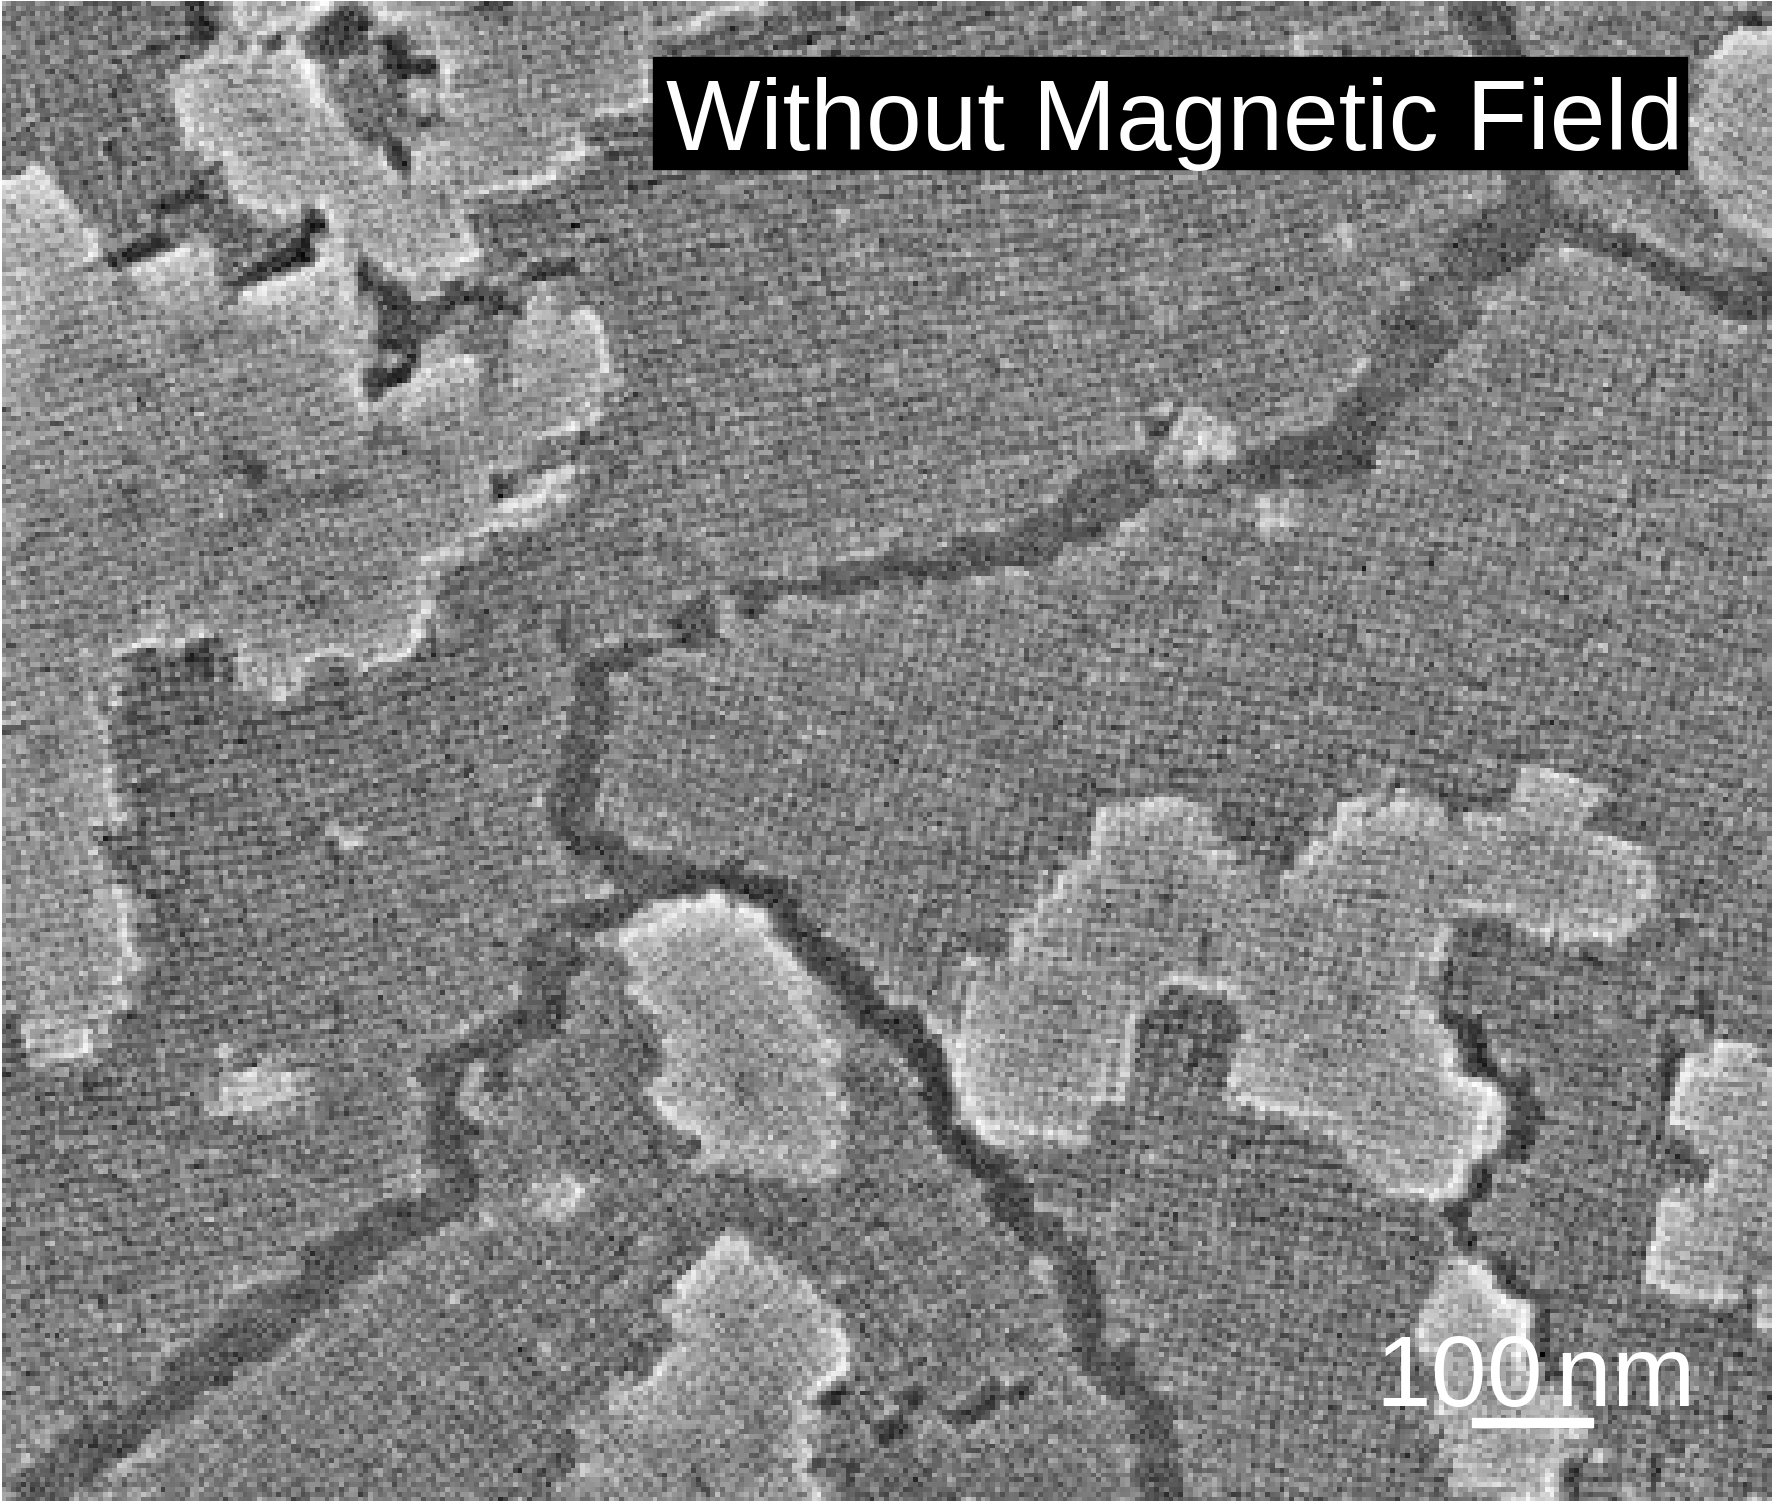
\includegraphics{monolayers_SEM_without_mag_field}
      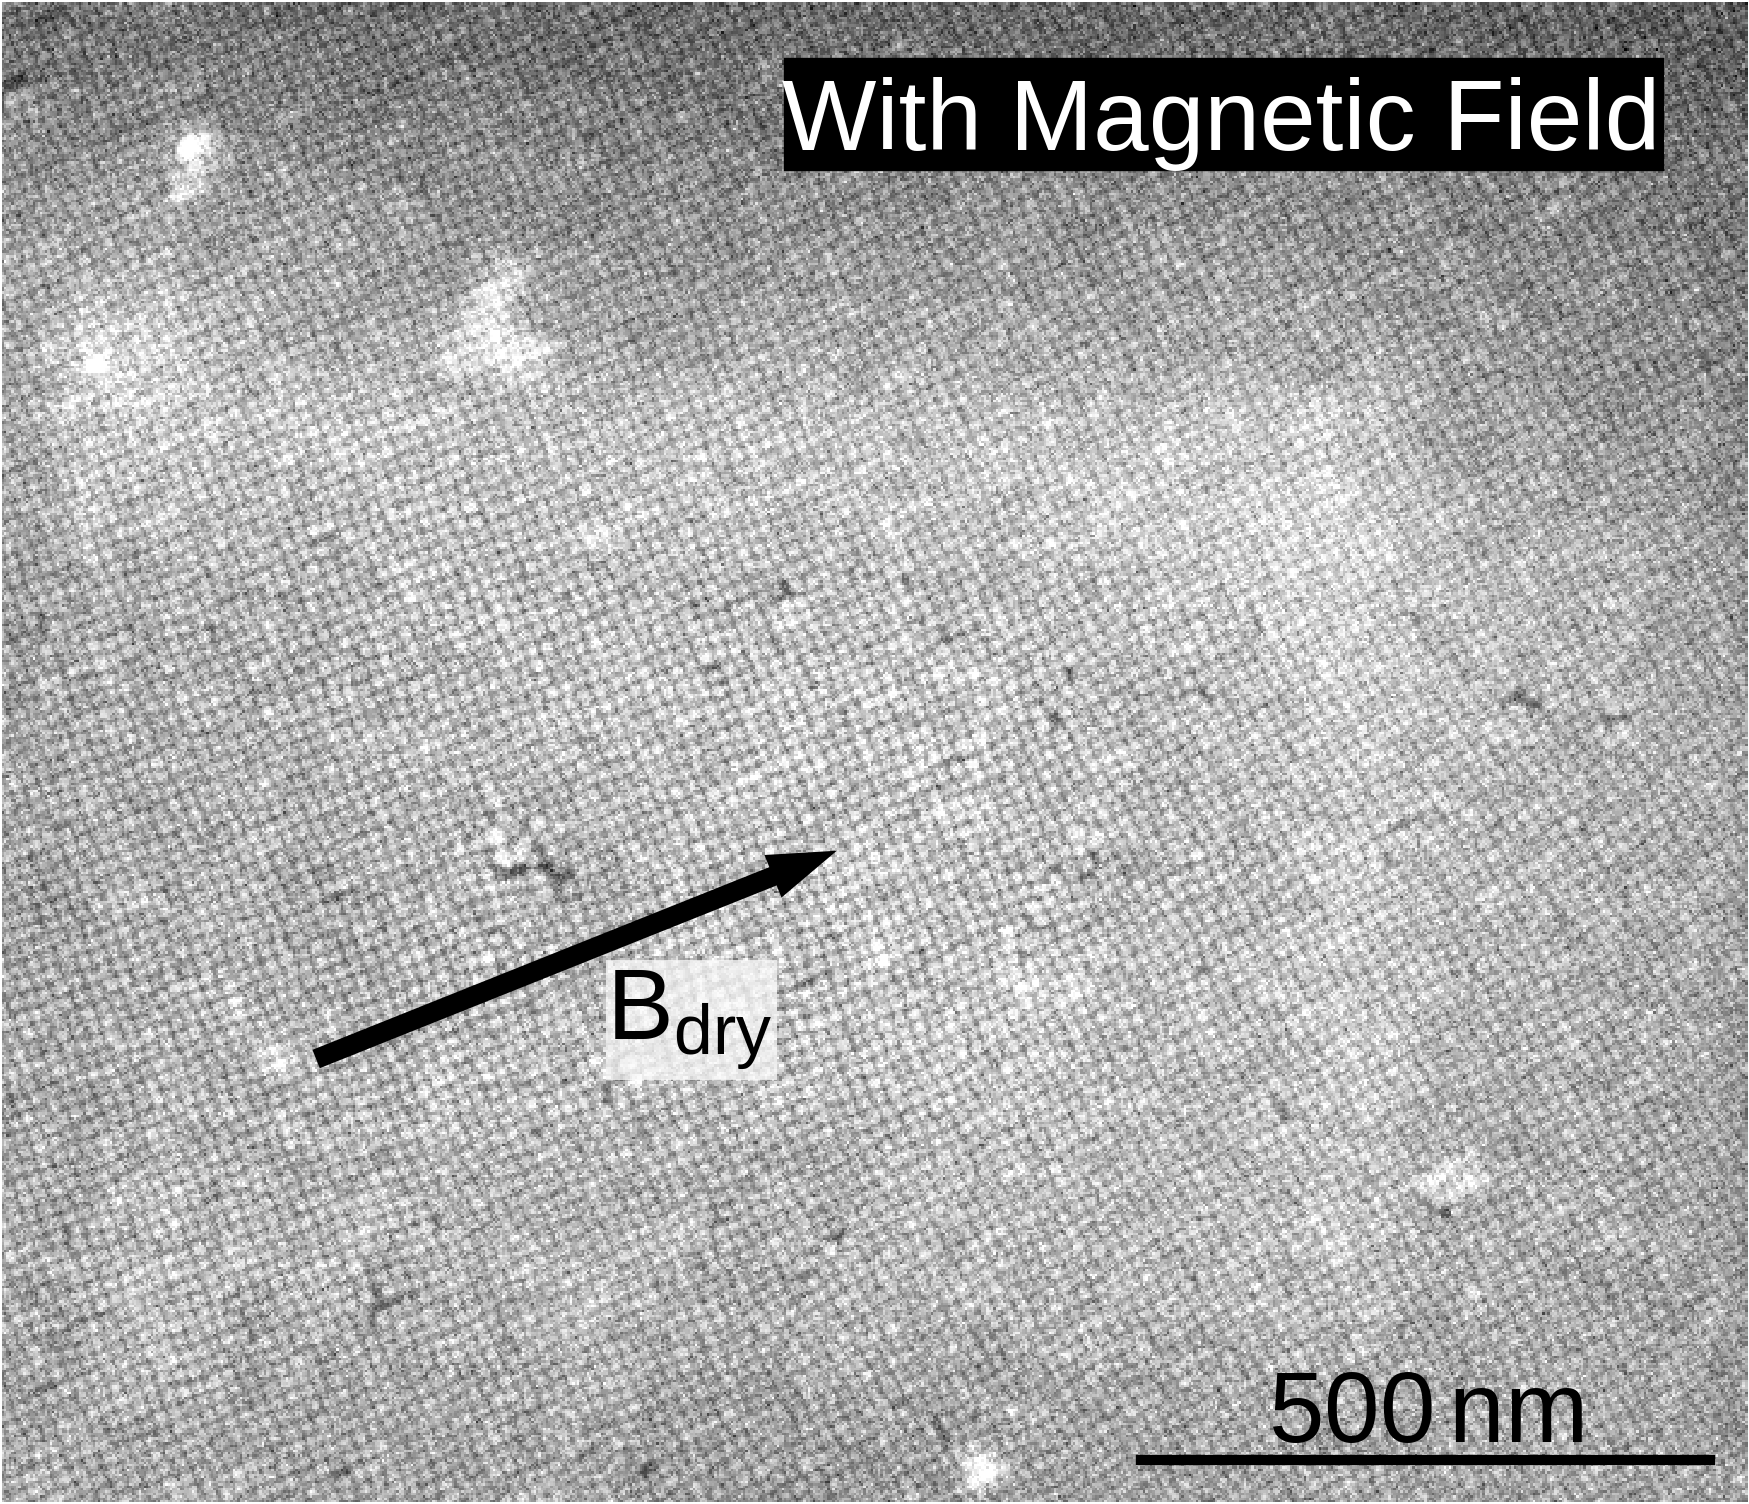
\includegraphics{monolayers_SEM_with_mag_field}
      \caption{\label{fig:monolayers:preparation:dryingConditions:magneticField}Comparison of simultaneously prepared monolayer from the same dispersion, one without applying a magnetic field, one within a Halbach cylinder with $B_{dry} \eq 40 \unit{mT}$.}
    \end{figure}
    A detailed quantitative study of these structures is, however, not in the scope of this work but left for future studies.

    For all presented samples in the following discussions, the first evaporation step is always performed at ambient conditions, in an open container, on an even surface, within a calm room as this has shown to provide the best results in all initial tests.

  \subsubsection{Second Stage: Slow Evaporating Components}
  \begin{figure}[tb]
    \centering
    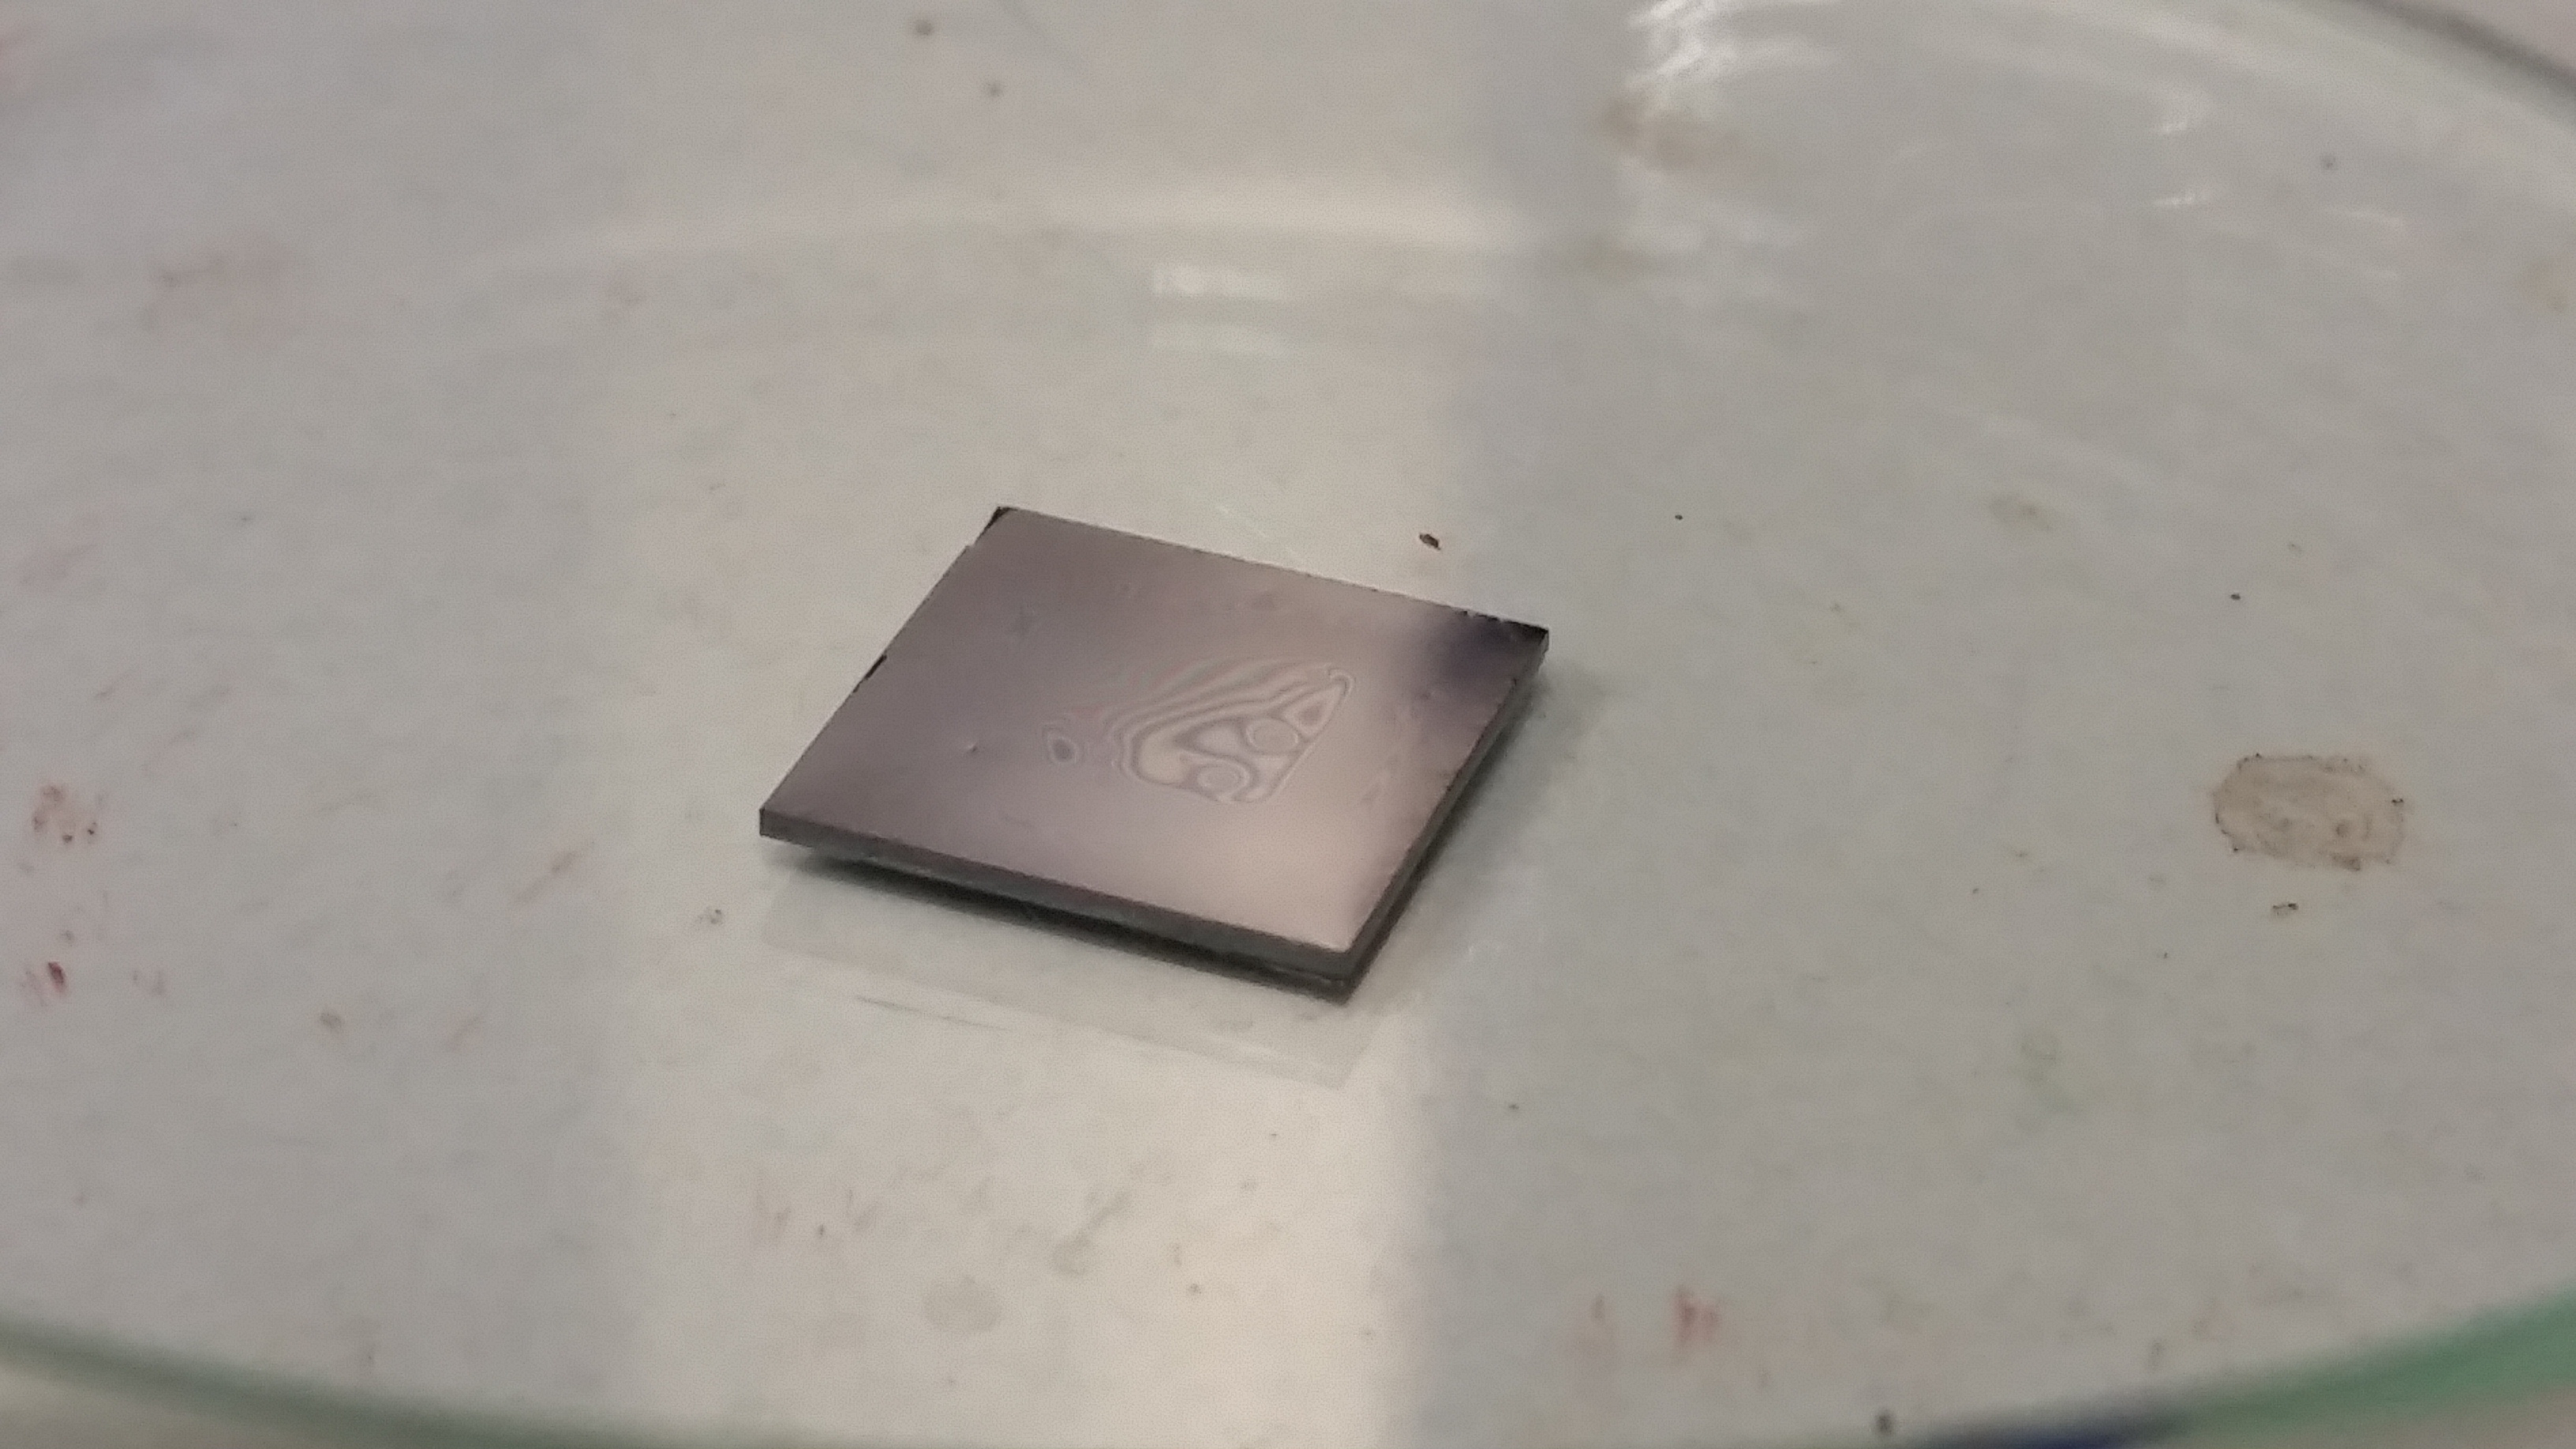
\includegraphics[width=0.7\textwidth]{monolayers_preparation_oilyFilm}
    \caption{\label{fig:monolayers:preparation:dryingConditions:oilyFilm}Thin oily film visible on a silicon wafer after the fast evaporating component of the dispersion has been dried during monolayer preparation.}
  \end{figure}
  After the fast evaporating component of the dispersion is dry, a thin oily film is visible on the wafer by thin-film interference as shown in \reffig{fig:monolayers:preparation:dryingConditions:oilyFilm}.
  Even after several weeks, the thin-film of 1-octadecene/oleic acid does not evaporate at ambient conditions and has to be removed actively at elevated temperatures.
  By successively increasing the temperature of an oven, it was found that a temperature of at least $140 \unit{^\circ C}$ is necessary to be applied to the monolayer for at least $6 \unit{h}$ to remove the organic components to most parts.
  Heating to this temperature quickly via a heating plate was found to be contraproductive as it leads to a inhomogeneous evaporation of the oily film.
  To have a homogeneous evaporation, the best found method is to place the substrate within a glass Petri dish that is covered with an aluminium foil that is perforated along the edge.
  The aluminium foil protects the wafer for one from dust and from other dirt in the oven, while it also directs the evaporating flow to controllably stream out the perforated edge.
  The best result is observed when the thin film of 1-octadecene/oleic acid is left within the oven at $80 \unit{^\circ C}$ for at least $12\unit{h}$ and then heated to $140 \unit{^\circ C}$ for at least $6\unit{h}$.
  It is important to note here that the oven needs to be properly balanced with a water level.
  Any slope of a few degrees leads to an accumulation at the lower side of the substrate as the gravitational force pulls the thin film to one side.

  When those steps are all considered, the second drying step leads to a homogeneous drying of most parts of the 1-octadecene/oleic acid.
  After this heating process, there is however often still some remaining organic components on the wafer surface that cannot be removed at $140 \unit{^\circ C}$, even when the sample is left for a week in the oven.
  One option is to increase the temperature even higher and be more aggressive in the evaporation of the organic solvents.
  However, attempts in that direction resulted in a reduced quality of the nanostructure.
  Therefore, a different approach was chosen, where the residues are washed away, which is described in the following.


\end{document}